\section{Conclusion}
In this paper we focus on the assistant decision task for airline capacity control under pandemic like COVID-19. We try to model the tradeoff between the satisfaction of passengers' transportation demand and the avoidance of any further disease spreading. Our model reflects such tradeoff well and shows the difficulty of striking a balance. For getting opitmal solution we use both the IBM CPLEX solver and the Differential Evolution Algorithm, and we could get satisfactory result in the latter way. However, to answer the quesiton about anarchy penalty, that is, the negative influence of a unregulated aviation industry under global pandemic, we should further study how the capacity of aviation network could influence the infection severity in different cities with airports.

To better illustrate the relationship between decision making with different dates/cities/$\epsilon$/$T$, we also apply echarts to our Dynamic Airline System in 3D, which can be visited online\footnote{\url{demo.network-economics.whiskychoy.com}}.

From figure 7(a) and 7(b) we can see with relaxation on parameter $T$, the width of the airlines apparently increases. From figure 7(b) and figure 7(d), we know only with relaxation on parameter $T$ and lower severity at Wuhan, a small proportion of the airline capacity from Wuhan is allowed to be recovered. Finally, we also visualize the airline capacity in absolute way, that is, use $C_{ij}$ rather than $C_{ij}/C_{ij}^{max}$, and we can see from figure 7(a) and 7(c) that the actual airline capacity between cities with low $d_{ij}$ is not that large.

\begin{figure}[H]
    \centering
    \subfigure[Relative $\epsilon=.7,T=1000$]{
        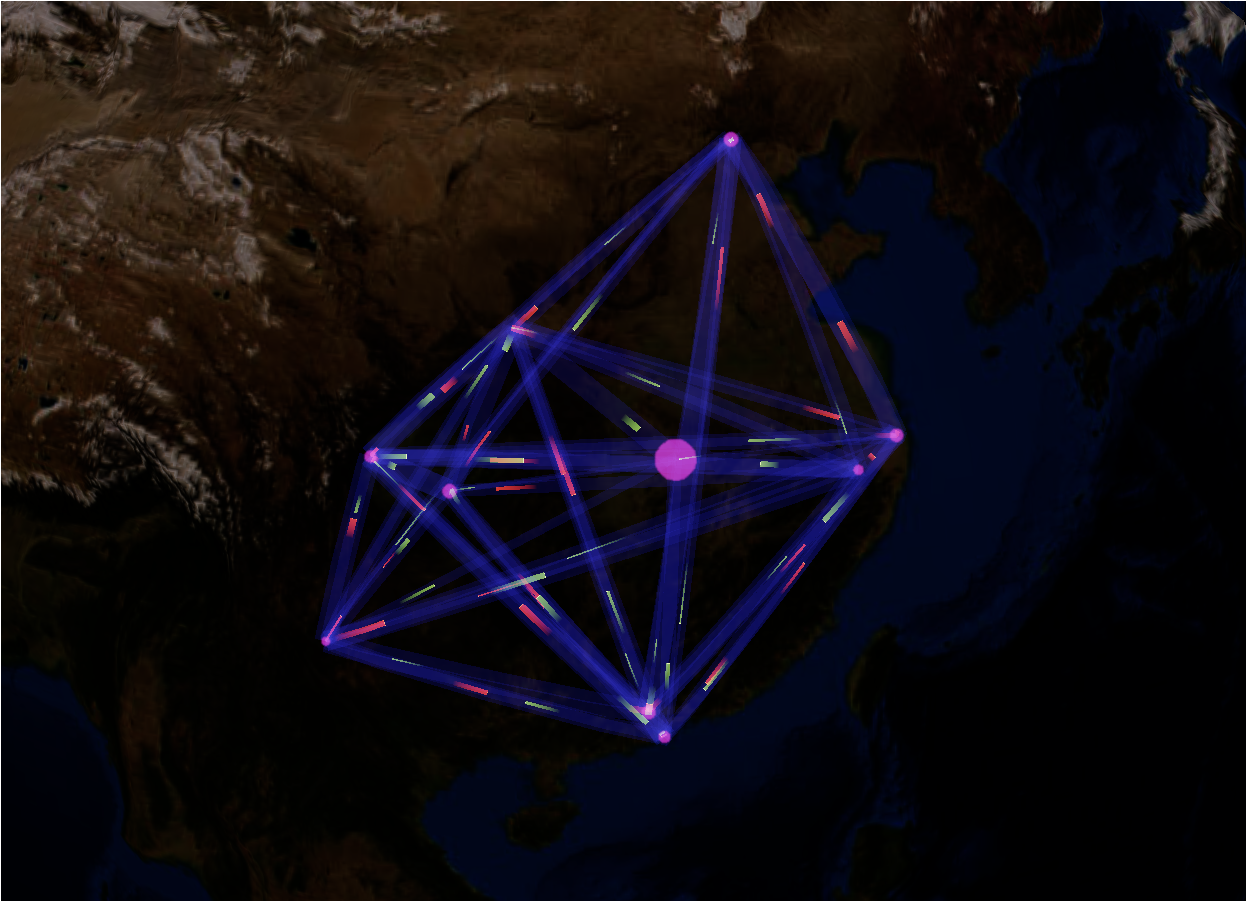
\includegraphics[width=0.46\columnwidth]{pic/relateive_T=1000_ep=0dot7_date=02162020.png}
    }
    \subfigure[Relative $\epsilon=.9, T=1000$]{
        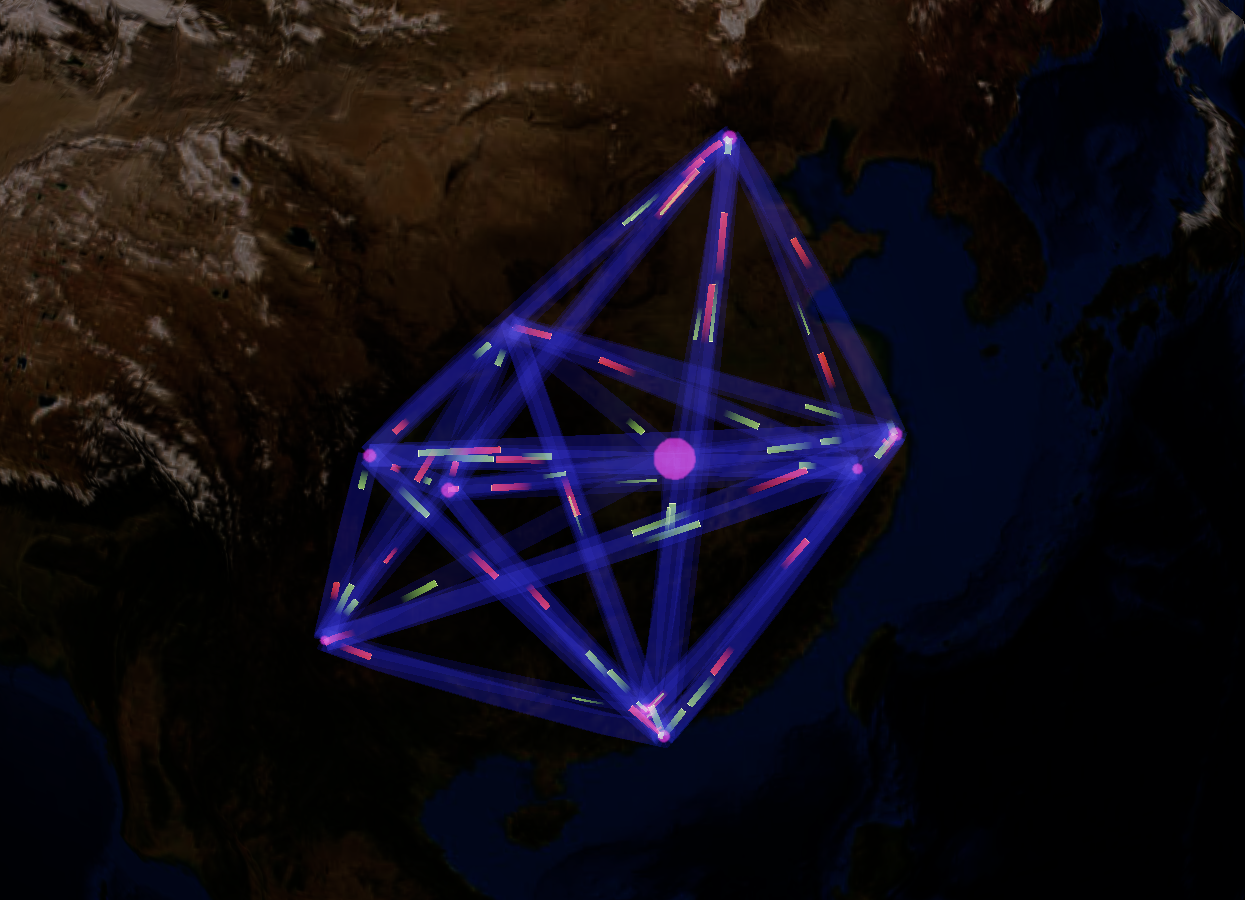
\includegraphics[width=0.46\columnwidth]{pic/relateive_T=1000_ep=0dot9_date=02162020.png}
    }
    \subfigure[Absolute $\epsilon=.7, T=1000$]{
        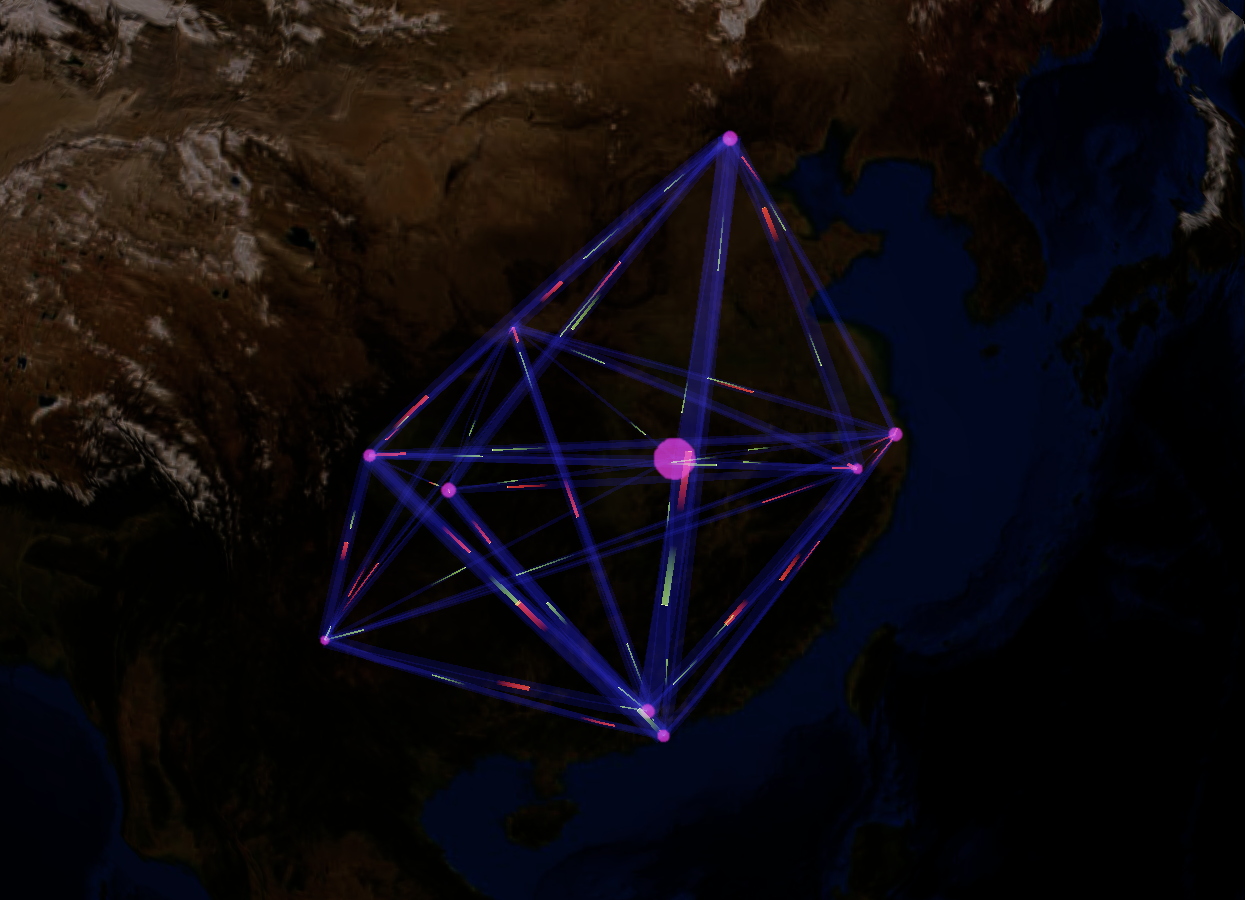
\includegraphics[width=0.46\columnwidth]{pic/absolute_T=1000_ep=0dot7_date=02162020.png}
    }
    \subfigure[Relative $\epsilon=.9, T=1000$]{
        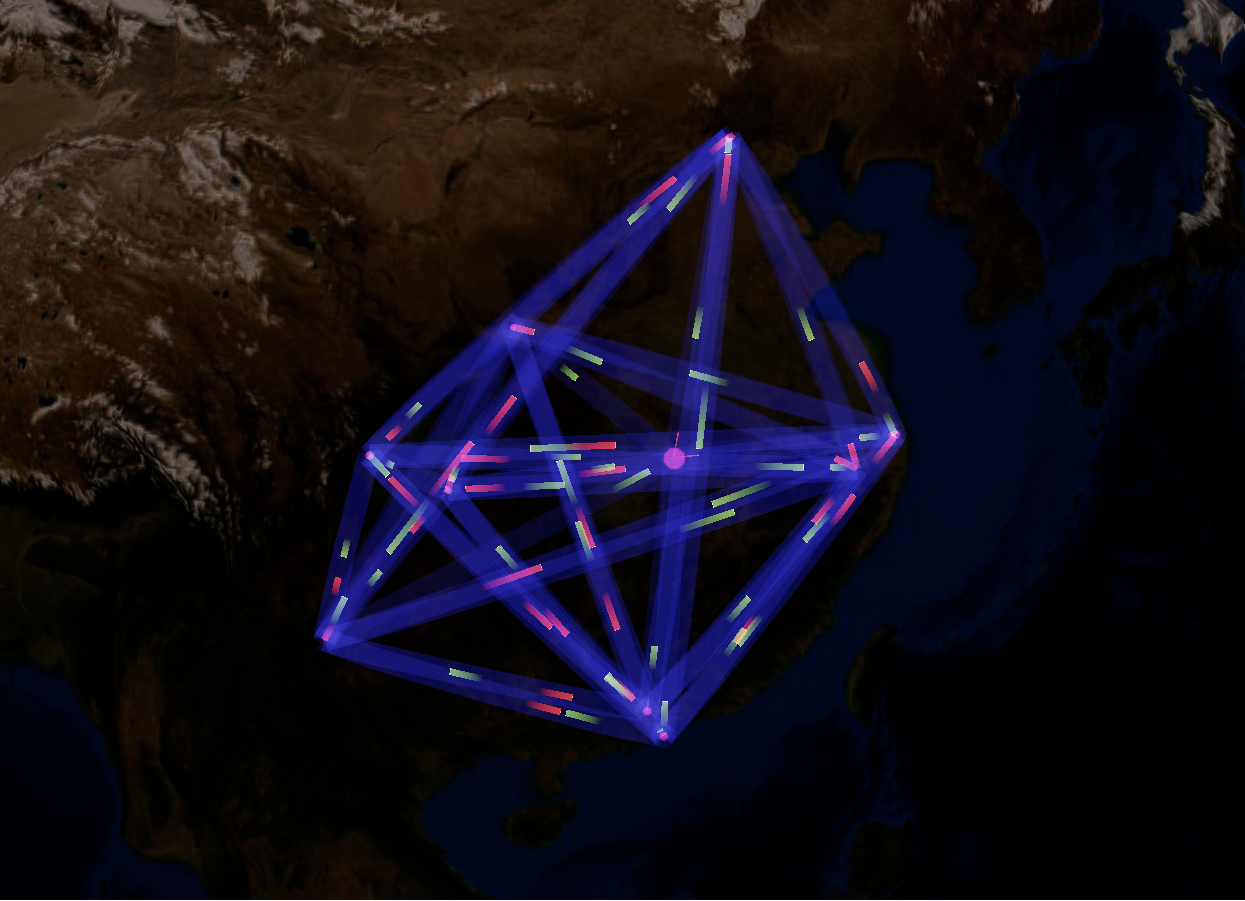
\includegraphics[width=0.46\columnwidth]{pic/relative_T=1000_ep=0dot9_date=04162020.png}
    }
    \caption{3D Airline System with Relative Capacity and Absolute Capacity. (a), (b): Feb. $16^{\rm th}$; (c), (d): Apr. $16^{\rm th}$}
    \label{fig:Convergence}
\end{figure}

% =================================